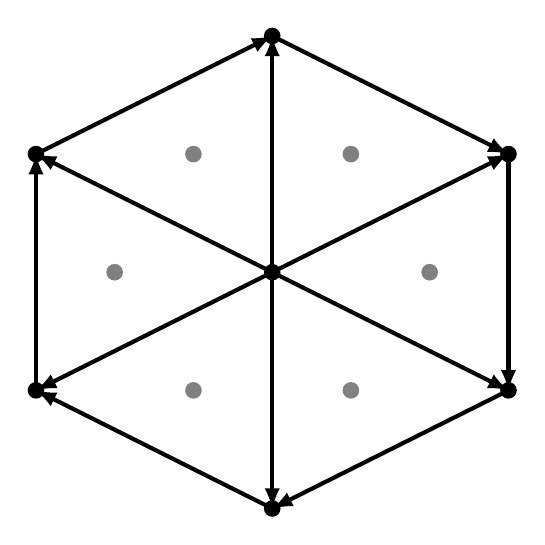
\begin{tikzpicture}[>=latex, line width=1.5pt, scale=1.5]
  % Coords
\coordinate (V0) at (2,0);
\coordinate (V1) at (2,2);
\coordinate (V2) at (0,1);
\coordinate (V3) at (4,1);
\coordinate (V4) at (4,-1);
\coordinate (V5) at (0,-1);
\coordinate (V6) at (2,-2);

%circumcenter
\coordinate (CC1) at (1.333,1);
\coordinate (CC0) at (2.666,1);
\coordinate (CC3) at (1.333,-1);
\coordinate (CC2) at (0.666,0);
\coordinate (CC4) at (2.666,-1);
\coordinate (CC5) at (3.333,0);

 
\coordinate (C01) at (2,1);
\coordinate (C02) at (1,0.5);
\coordinate (C03) at (3,0.5);
\coordinate (C05) at (1,-0.5);
\coordinate (C04) at (3,-0.5);
\coordinate (C06) at (2,-1);

\coordinate (C12) at (1,1.5);
\coordinate (C25) at (0,0);
\coordinate (C56) at (1,-1.5);
\coordinate (C46) at (3,-1.5);
\coordinate (C34) at (4,0);
\coordinate (C13) at (3,1.5);

%\fill[black, opacity=0.3] (CC0) -- (CC1) -- (CC2) -- (CC3) -- (CC4) -- (CC5) -- (CC0);
%\fill[black, opacity=0.3] (V0) -- (CC5) -- (CC0) -- (V0);
%\fill[opacity=0.4]  (V1) -- (V3) -- (V4) -- (V6) -- (V5) -- (V2);
  % Arrows\tilde{\sigma}
\draw[->](V0) -- (V1);
\draw[<-](V1) --  (V2);
\draw[->](V0) -- (V2);
\draw[->](V1) --  (V3);
%\draw[blue,->](V0) -- (V3);
\draw[->](V0) -- (V3);
\draw[->](V0) -- (V4);
\draw[->](V0) -- (V5);
\draw[->](V5) --  (V2);
\draw[->](V3) --  (V4);
\draw[->](V4) -- (V6);
\draw[->](V0) -- (V6);
\draw[->](V6) -- (V5);
 
\begin{scope}[gray,  line width=1pt]
  %\draw[->] (CC0) -- (CC1);
  %\draw[->] (CC1) -- (CC2);
  %\draw[->] (CC2) -- (CC3);
  %\draw[->] (CC3) -- (CC4);
  %\draw[->] (CC4) -- (CC5);
  %\draw[->] (CC5) -- (CC0);
  %\draw[<-,densely dotted] (C12) -- (CC1);
  %\draw[<-,densely dotted] (C25) -- (CC2);
  %\draw[<-,densely dotted] (C56) -- (CC3);
  %\draw[<-,densely dotted] (C46) -- (CC4);
  %\draw[<-,densely dotted] (C34) -- (CC5);
  %\draw[<-,densely dotted] (C13) -- (CC0);
%\draw[dotted] (CC1) -- (CC4);
%\draw[dotted] (CC2) -- (CC5);
%\draw[dotted] (CC3) -- (CC0);

%\draw[dotted] (CC1) -- (V1);
%\draw[dotted] (CC2) -- (V2);
%\draw[dotted] (CC3) -- (V5);
%\draw[dotted] (CC4) -- (V6);
%\draw[dotted] (CC5) -- (V4);
%\draw[dotted] (CC0) -- (V3);
%
%\draw[dotted] (CC1) -- (V2);
%\draw[dotted] (CC2) -- (V5);
%\draw[dotted] (CC3) -- (V6);
%\draw[dotted] (CC4) -- (V4);
%\draw[dotted] (CC5) -- (V3);
%\draw[dotted] (CC0) -- (V1);

%\draw[blue,->] (CC5) -- (CC0); 

\fill (CC0) circle (2pt);
\fill (CC1) circle (2pt);
\fill (CC2) circle (2pt);
\fill (CC3) circle (2pt);
\fill (CC4) circle (2pt);
\fill (CC5) circle (2pt);

%
%
%\fill (C01) circle (2pt);
%\fill (C02) circle (2pt);
%\fill (C03) node[right, blue] {\(\ e\)}circle (2pt);
%\fill (C05) circle (2pt);
%\fill (C04) circle (2pt);
%\fill (C06) circle (2pt);
% 
%
%\fill (C12) circle (2pt);
%\fill (C25) circle (2pt);
%\fill (C56) circle (2pt);
%\fill (C46) circle (2pt);
%\fill (C34) circle (2pt);
%\fill (C13) circle (2pt);
\end{scope}

\fill[] (V0) circle (2pt);
%\fill[] (V0) node[left] {\(v\ \)} circle (2pt);
\fill (V1) circle (2pt);
\fill (V2) circle (2pt);
\fill (V3) circle (2pt);
\fill (V4) circle (2pt);
\fill (V5)circle (2pt);
\fill (V6)circle (2pt);



\end{tikzpicture}

